%% This is an example first chapter.  You should put chapter/appendix that you
%% write into a separate file, and add a line \include{yourfilename} to
%% main.tex, where `yourfilename.tex' is the name of the chapter/appendix file.
%% You can process specific files by typing their names in at the 
%% \files=
%% prompt when you run the file main.tex through LaTeX.
\chapter{Design Tools}
\todo{introduction to design tools}

\section{Codeable Objects}
Codeable Objects is computational design tool that allowed people to design a laser cut lamp. The choice of a lamp allowed for a relatively broad design space wherein aesthetics were a primary consideration, while still retaining the qualities of functionality and utility in the finished product.  Lamps possess an established function, but offer a great deal of flexibility and personal freedom in the aesthetics and form. In addition, there is an established history of creating DIY lamps via digital fabrication. The Instructables community tutorial website has an entire section devoted to DIY lamps, and many examples of patterns that use a laser cutter for fabrication. 
\begin{center}
\begin{figure}[h!]
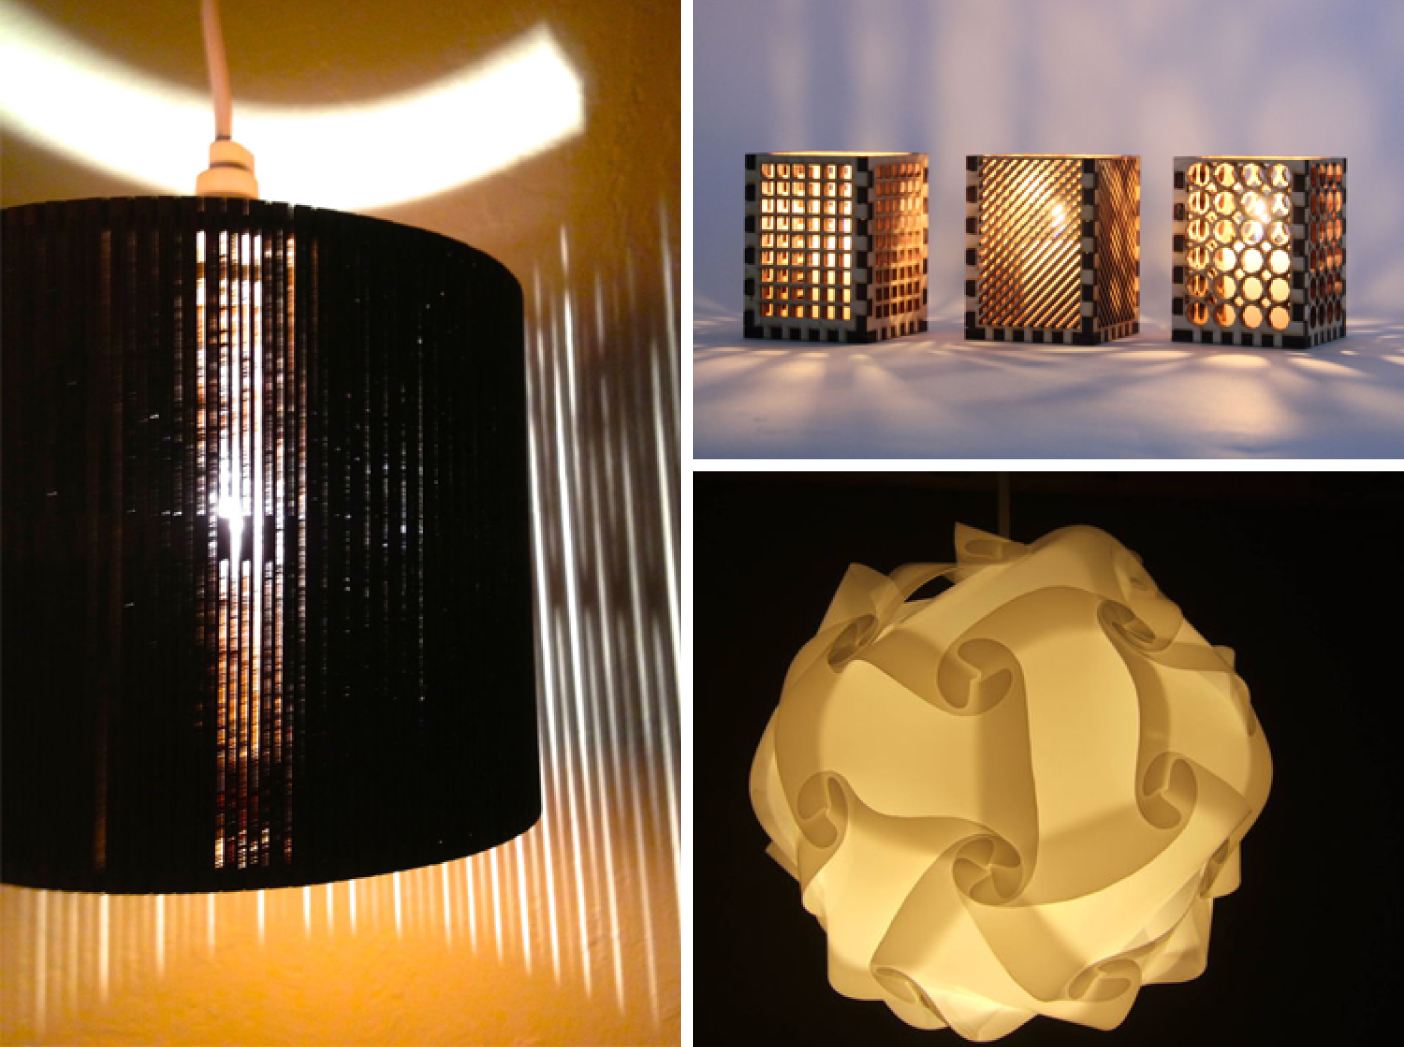
\includegraphics[width=6.5in]{images/instructables_lamps.png}
\caption{a selection of laser cut lamps from Instructables}
\end{figure}
\end{center}
\subsection{Motivation}
One of the restrictions of many of these examples is that they require the person making the lamp to directly emulate the design provided by the creator of the tutorial. If the person wishes to deviate from the original design, they  need to use a CAD tool like Adobe Illustrator or Solid Works\cite{instructables_lamp_1}. As mentioned in Section \ref{sec:professional_computational_design_tools}, professional CAD tools like Solid Works are often difficult to access and use for casual practitioners. In addition, during my personal experience in using a non-parametric tool like illustrator to design, I often found I had to resort to fabricating numerous sample pieces of in order to ensure the joints and form would function correctly in the final piece. If I made a mistake, or decided I wanted to modify the design, I lost time and materials in the fabricating process, and had to endure the tedious process of adjusting correcting each individual part. 
\begin{center}
\begin{figure}[h!]
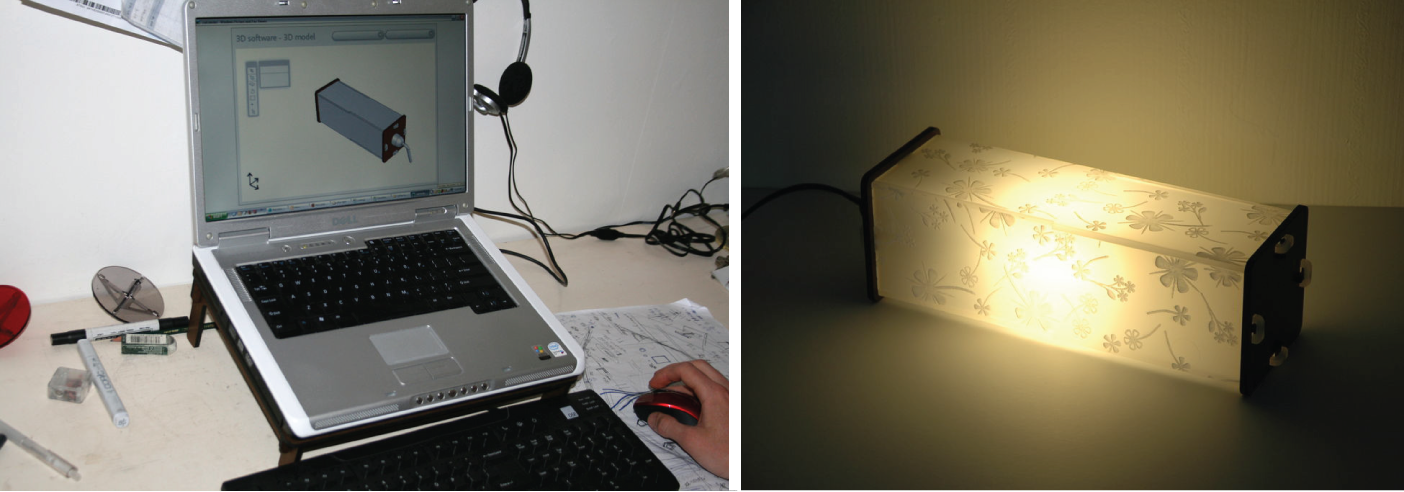
\includegraphics[width=6.5in]{images/solidworks_lamp.png}
\caption{Instructables lamp tutorial with SolidWorks design process}
\end{figure}
\end{center}
One of the most frequent applications of a laser cutter is to create 3D forms by assembling 2D press fit pieces in a frame-like structure. I found that when creating 3D forms that were curved, it was extremely challenging in traditional 2D CAD software to correctly size and design parts which would fit the faces of the form. This was particularly relevant to lamp design, wherein it was necessary to create shades to diffuse the light. The shades also provided an excellent space for incorporating styles and patterns into the lamp. The combined tasks of simplified design and customization, parametric manipulation, and the calculation and conversion of a 3D form to 2D parts indicated that computational design would be a good match for the task of designing and fabricating a laser cut lamp. 
	
\subsection{Tool Description and workflow}
The objective of the first version of Codeable Objects was simple: to create a tool that allowed to design a custom lamp by describing the form and the pattern of the shades, which they could then fabricate and assemble. The lamp itself was comprised of 4 basic parts, a wooden press fit frame, a set of vellum pieces that fit over the frame to act as a shade,a set of cardstock pieces with a pattern that fit over the shades, and a commercial made light fixture that fit into the frame (see figure: \ref{fig:lamp_parts}.)
\begin{center}
\begin{figure}[h!]
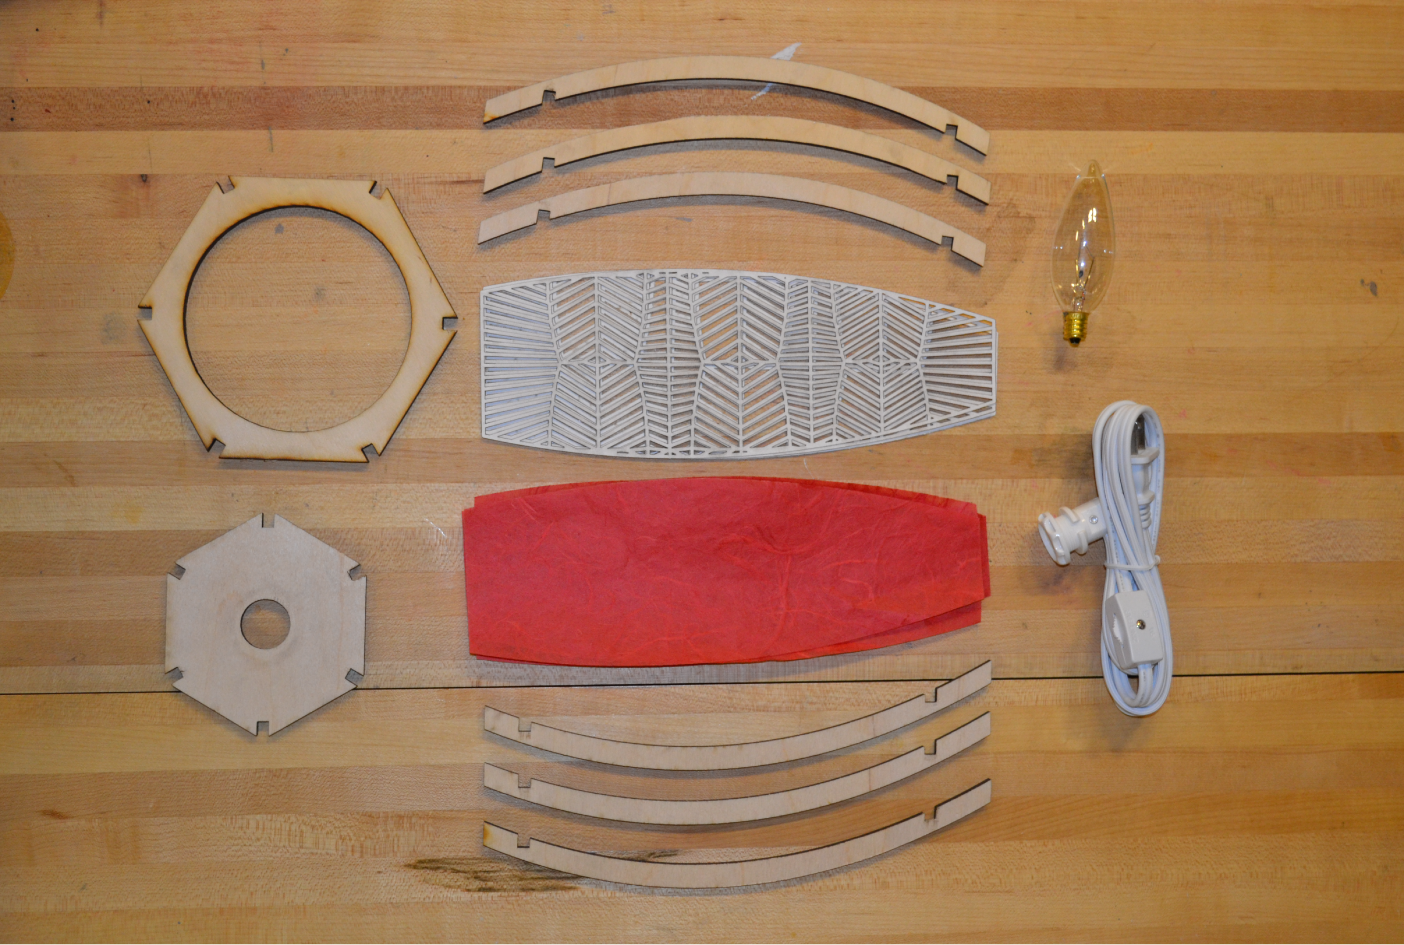
\includegraphics[width=5.337in]{images/parts.png}
\caption{the individual parts of a lamp}
\label{fig:lamp_parts}
\end{figure}
\end{center}
Codeable Objects was developed as a programing library for Processing andcontained a set of pre-defined programing methods that allow the user to describe the lamp, and define the tool paths for all three materials. For the first version of the library, all design took place via textual programing. Within the Processing IDE one imports and initialize the controller class of the library, and uses it to call four main functions that determine the height, top width, middle width and bottom width of the lamp. These 4 parameters are used to determine the form of the lamp, by generating the equation of a parabola with 3 intersection points. By rotating this parabola round the y-axis, it was possible to generate a closed 3-dimensional ellipsoid form.  The library also provided access to an additional set of methods that control over a number of other parameters in describing the form of the lamp, including the number of sides, the resolution of the curve and the position of the internal structural supports.  When the code is compiled, the application displays a graphic view containing 3d wireframe model of the current lamp as defined by the parameters. 


		Workflow description
		Workshop
		Workshop results

	\section{Soft Objects}
		Motivation and design principles
		Tool Description
		Workflow description
		Workshop
		Workshop results
		
	\section{DressCode}
		Motivation and design principles
		Tool Description
		Workflow description
		Workshop
		Workshop results
		Curriculum building
		Curriculum results
